\chapter{Métodos de clasificación}
\section{Selección de palabras clave de una categoría}
\label{sec:atributos}


Para determinar que palabras son las más representativas dentro de una categoría, buscamos aquellas palabras que se usan con más frecuencia dentro de cada categoría, una vez las tengamos las utilizaremos para clasificar aquellas noticias que no se encuentran recogidas bajo ninguna categoría. Para crear estos grupos de palabras utilizaremos las noticias que previamente hemos almacenado y conocemos su categoría, aproximadamente unos 50000 ejemplos de texto.

\subsection{Método propuesto}

Lo primero es crear una lista con todas las palabras que aparecen en las noticias de una determinada categoría eliminando determinadas palabras que no son importantes para la categoría a pesar de poder ser muy común encontrarla en los textos. 

El criterio para eliminar estas palabras es el siguiente, tenemos una lista con una serie de palabras como pronombres, preposiciones, otras palabras de uso común, nombres propios y nombres de municipios. La razón de eliminar nombres propios y nombres de municipios es que encontramos referencias al pueblo, a la provincia o a personas que ostentan distintos cargos públicos en la mayoría de los textos por lo que acaban siendo palabras muy comunes que no aportan significado a la categoría donde se encuentran.

Tras este primer filtrado tenemos un segundo proceso en el que eliminamos caracteres numéricos, algunos caracteres de control y aquellas palabras que no superen los tres caracteres, la razón para esto es que las palabras con esa longitud que acaban como palabras comunes y por ello representativas de la categoría son en realidad números romanos, que hacen referencia a algún tipo de evento, o abreviaturas como tlf, ext, o m.

Una vez tenemos la lista con las palabras candidatas generamos un diccionario a partir de dicha lista y así tener una estructura de datos donde la clave es la propia palabra y el valor es el número de apariciones de la palabra.

Una vez generados todos los diccionarios, uno por categoría, vamos iterando la lista de diccionarios. Para cada diccionario sacamos una lista con todas las claves y estudiamos como es de representativa cada palabra en todas las categorías. Para ello generaremos un vector en el que almacenamos como de común es la palabra que estamos estudiando en cada categoría. Pero como no tenemos un número de noticias igual en cada categoría necesitamos una medida relativa para poder comparar, por lo que dividimos el número de apariciones entre el número de noticias de esa categoría y obtenemos el número medio de apariciones de una palabra por noticia. 

A continuación dividimos entre el máximo valor de la lista y multiplicamos por mil para normalizarla y poder tener una medida que como de común es la palabra dentro de la categoría con valores de cero a mil. Valores cercanos a cero indican palabras poco representativas y valores cercanos a mil indican palabras muy comunes. En este punto calculamos el valor medio del vector ya que un valor medio alto nos indica que la palabra es muy común en la mayoría de las categorías por lo que no aporta nada a ninguna categoría en particular, en este caso la palabra se elimina de todas las categorías donde aparezca. El siguiente paso es ver como es de común la palabra en el diccionario que se está estudiando comparando con el valor mayor valor, es decir la categoría donde la palabra es más común. Para ello utilizamos la diferencia relativa entre dos números con la siguiente formula.


\begin{equation}
  diferencia(X,Y) = \frac{X - Y}{MAX(X,Y)} \times 1000
\end{equation}


Con esta fórmula obtenemos valores entre menos mil y mil, valores cercanos a menos mil indican que Y es muy distinto y mayor que X, valores cercanos a cero indican números muy parecidos y valores cercanos a mil indican que X es muy distinto y mayor que Y. Por lo que si comparamos siendo X el mayor valor del vector y Y el valor del vector que estamos estudiando, si obtenemos un valor cercano a mil estamos ante el caso de que la palabra en la categoría actual es muy poco representativa en comparación con el máximo por lo que eliminamos la palabra de la categoría actual.

\subsubsection{Experimentación y resultados}

Si tomamos los datos anteriores y creamos un grafo conectando palabras y categorías, asignando un peso a cada arista igual al valor de frecuencia calculado anteriormente obtenemos el siguiente ejemplo:


\begin{figure}[h]
\begin{center}
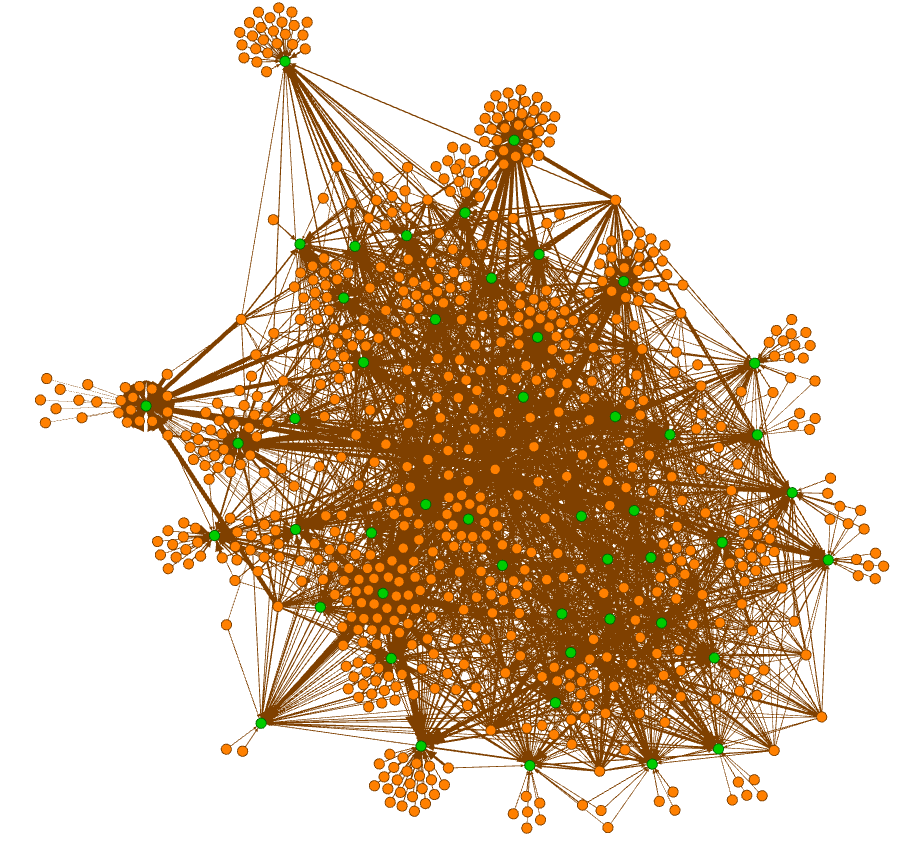
\includegraphics[scale=0.5]{Categorias/palabras_clave/grafocompleto.png} 
\caption{Grafo palabras y categorías}
\end{center}

\end{figure}

En este grafo vemos en color verde aquellos nodos que representan una categoría y en naranja las palabras. Cada categoría se rodea de aquellas palabras que son relevantes para ella. 

A continuación se muestra el ejemplo de la categorías Festejos y Tráfico para mostrar como las palabras se organizan al rededor de sus categorías.
%\begin{center}
%\begin{figure}[h]
%	\centering	
%	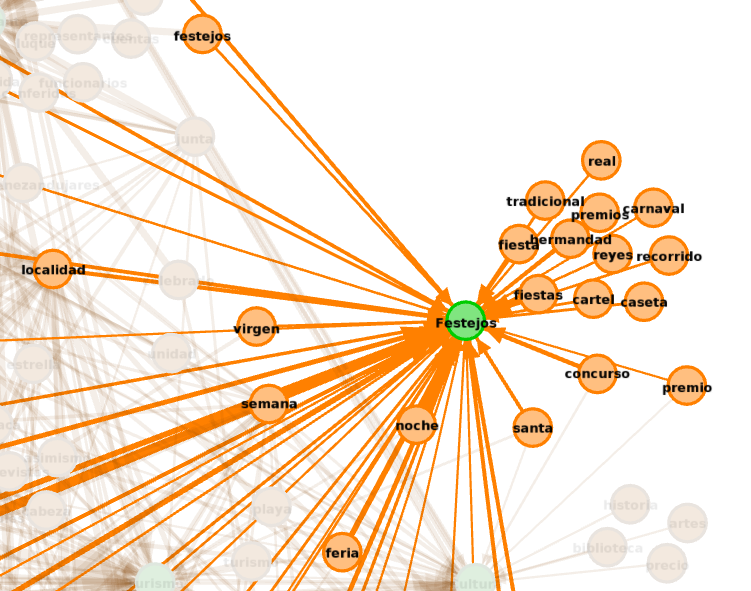
\includegraphics[scale=0.4]{Categorias/palabras_clave/festejos.png} 		
%	\caption{Palabras relevantes para la categoría Festejos}
%\end{figure}
%\end{center}
 

\begin{figure}[h]
	\centering
	\begin{subfigure}[b]{0.54\textwidth}
		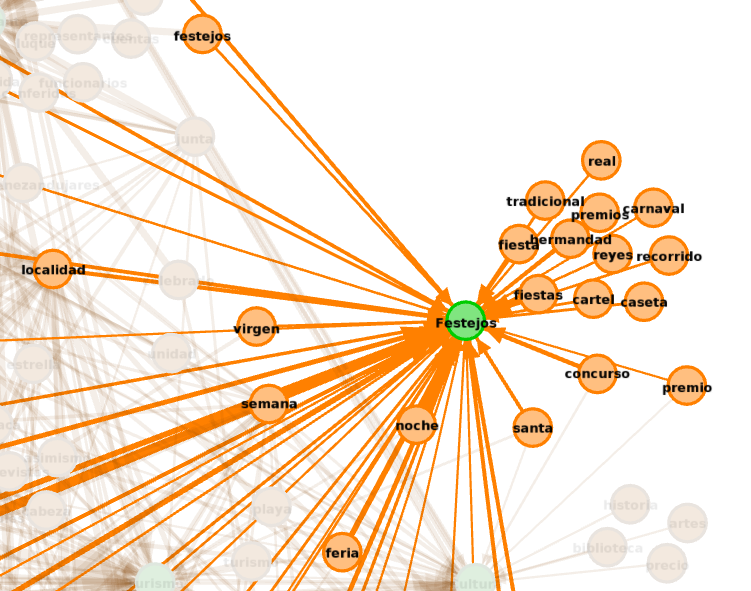
\includegraphics[scale=0.3]{Categorias/palabras_clave/festejos.png} 
		\caption{Palabras relevantes para la categoría Festejos}
	\end{subfigure} 
	\begin{subfigure}[b]{0.44\textwidth}
		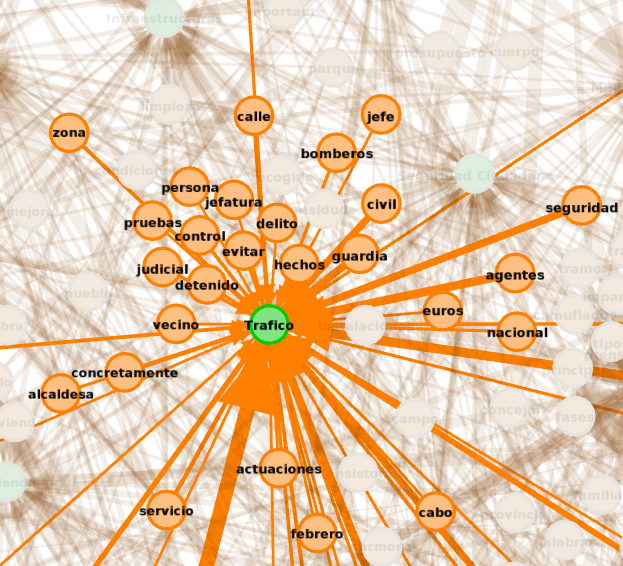
\includegraphics[scale=0.3]{Categorias/palabras_clave/trafico.png} 
		\caption{Palabras relevantes para la categoría Tráfico}
	\end{subfigure}
\end{figure}









Categorías que representen conceptos similares y que por ello también comparten muchas palabras también quedan cerca. Como es el caso de las categorías Igualdad, PIM (Punto de información de la mujer) y Mujer.


\begin{figure}[!htbp]
\begin{center}
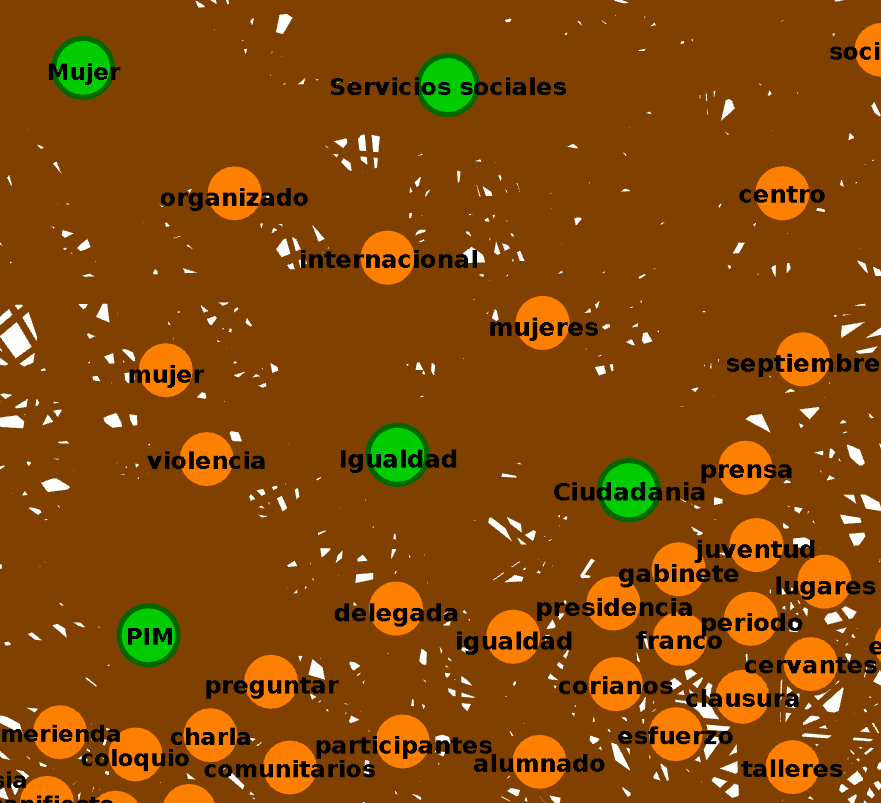
\includegraphics[scale=0.33]{Categorias/palabras_clave/cat_similares.png} 
\caption{Grafo palabras y categorías}
\end{center}
\end{figure}



\subsection{Aproximación TF-IDF}

Otra forma de determinar que palabras son relevantes para una categoría es la aplicación del algoritmo TF-IDF. Este algoritmo se divide en dos partes, la primera es la frecuencia del termino, esto es simplemente el número de veces que una palabra aparece en el documento. La segunda parte es la frecuencia inversa en el documento, con esto se intenta crear un factor de corrección para aquellas palabras que aparecen con mucha frecuencia en muchos documentos.

Desde un punto de vista matemático podemos definirlo como:
\begin{equation}
  TF-IDF(w,d) = TF \times IDF(w,D)
\end{equation}
La frecuencia de términos es el número de veces que el termino $w$ aparece en el documento $d$
La frecuencia inversa de documentos determina como de común es el termino $w$ dentro del conjunto de documentos $D$

\begin{equation}
  IDF(w,D) = log(\frac{N}{\|\{d \in D : w \in d \}\|})
\end{equation}